\section{Zadanie 2}

\subsection{Grupowanie}

\subsubsection{Implementacja}

\subsubsection{Wyniki}

\begin{figure}[H]
	\centering
	\hspace*{-0.8in}
	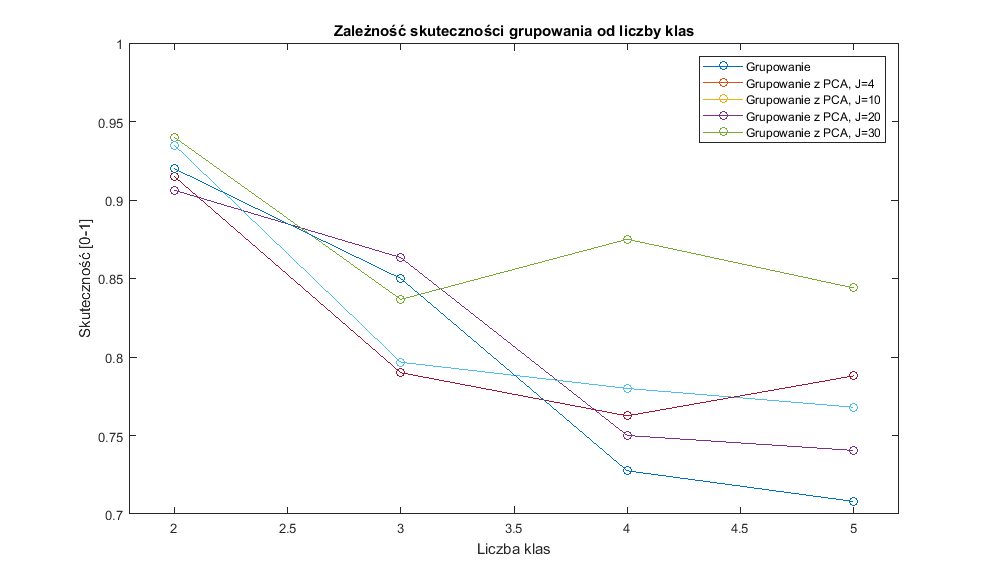
\includegraphics[scale = 0.7]{img/acc_from_classes_group.png}
	\caption{Skuteczność grupowania dla wymiarów pełnych i zredukowanych}  
	\label{rys:acc_from_classes_group} 
\end{figure}

\begin{figure}[H]
	\centering
	\hspace*{-0.8in}
	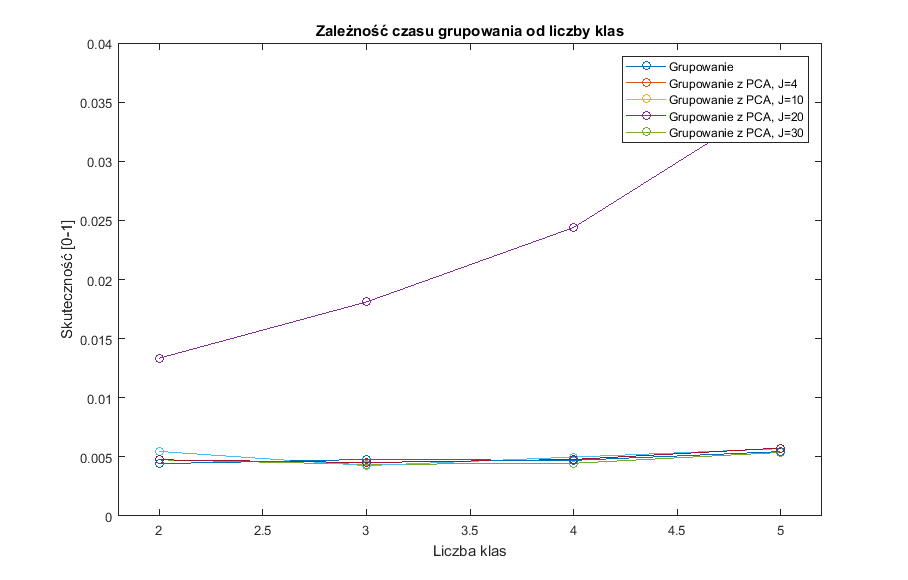
\includegraphics[scale = 0.7]{img/time_from_classes_group.png}
	\caption{Czas grupowania dla wymiarów pełnych i zredukowanych}  
	\label{rys:time_from_classes_group} 
\end{figure}


\subsection{Klasyfikacja}

\subsection{Porównanie klasyfikacji i grupowania}}

\begin{figure}[H]
	\centering
	\hspace*{-0.8in}
	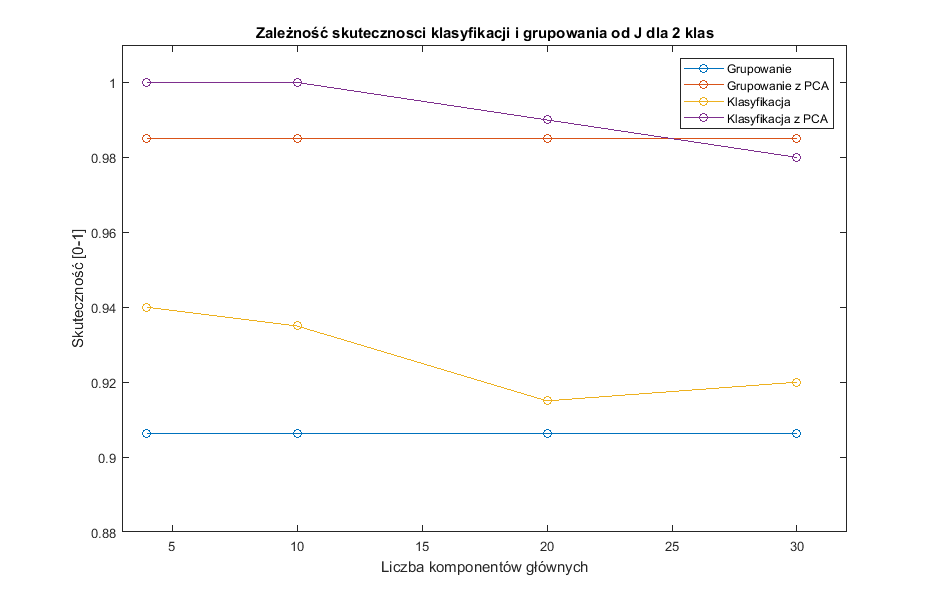
\includegraphics[scale = 0.7]{img/acc_from_J_2classes.png}
	\caption{Skuteczność grupowania i klasyfikacji dla 2 klas}  
	\label{rys:acc_from_J_2classes} 
\end{figure}

\begin{figure}[H]
	\centering
	\hspace*{-0.8in}
	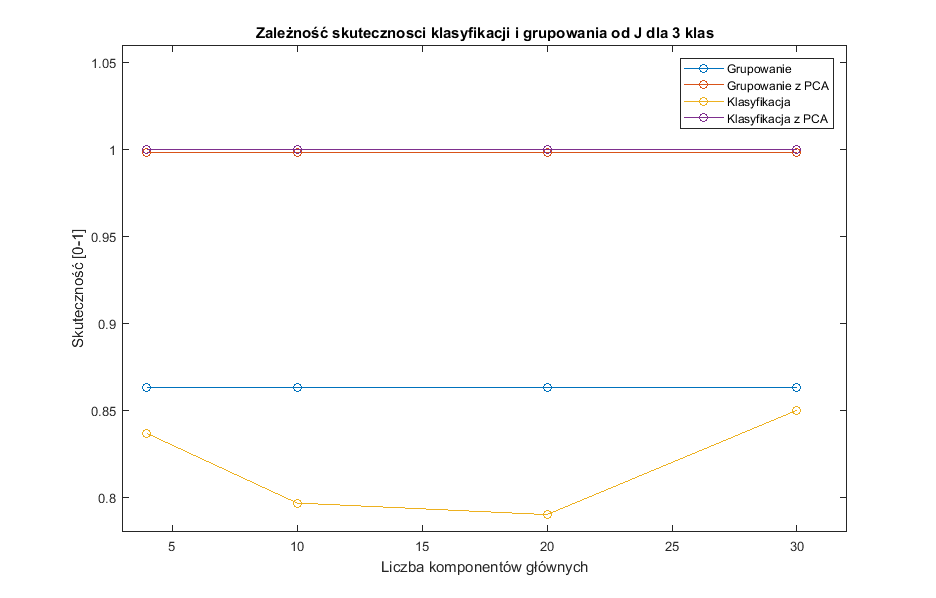
\includegraphics[scale = 0.7]{img/acc_from_J_3classes.png}
	\caption{Skuteczność grupowania i klasyfikacji dla 3 klas}  
	\label{rys:acc_from_J_3classes} 
\end{figure}

\begin{figure}[H]
	\centering
	\hspace*{-0.8in}
	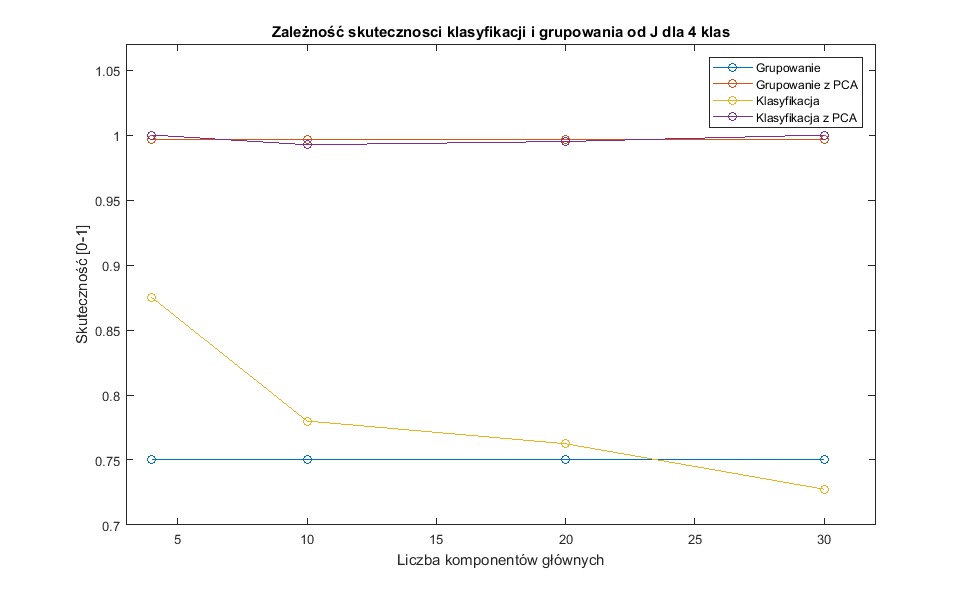
\includegraphics[scale = 0.7]{img/acc_from_J_4classes.png}
	\caption{Skuteczność grupowania i klasyfikacji dla 4 klas}  
	\label{rys:acc_from_J_42classes} 
\end{figure}

\begin{figure}[H]
	\centering
	\hspace*{-0.8in}
	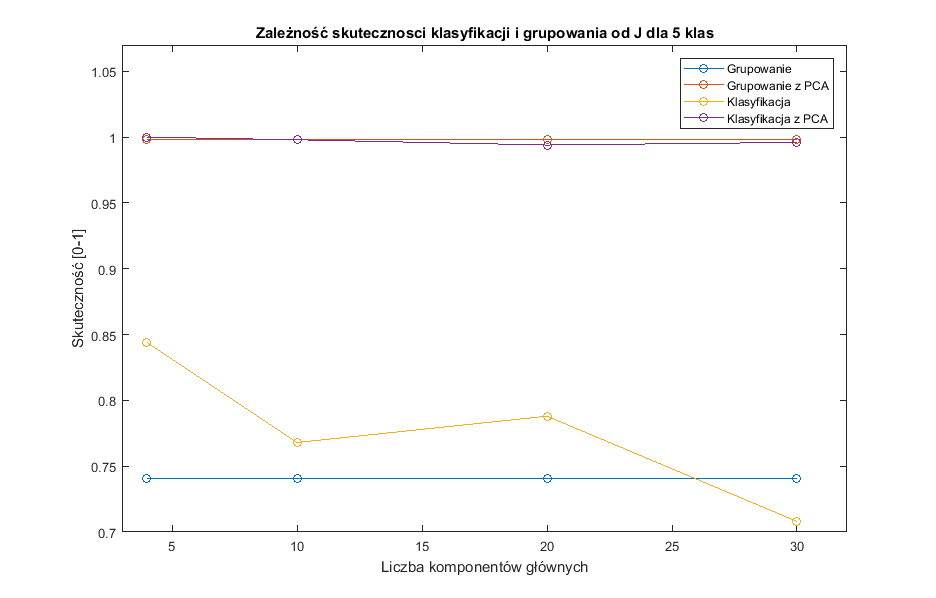
\includegraphics[scale = 0.7]{img/acc_from_J_5classes.png}
	\caption{Skuteczność grupowania i klasyfikacji dla 5 klas}  
	\label{rys:acc_from_J_5classes} 
\end{figure}